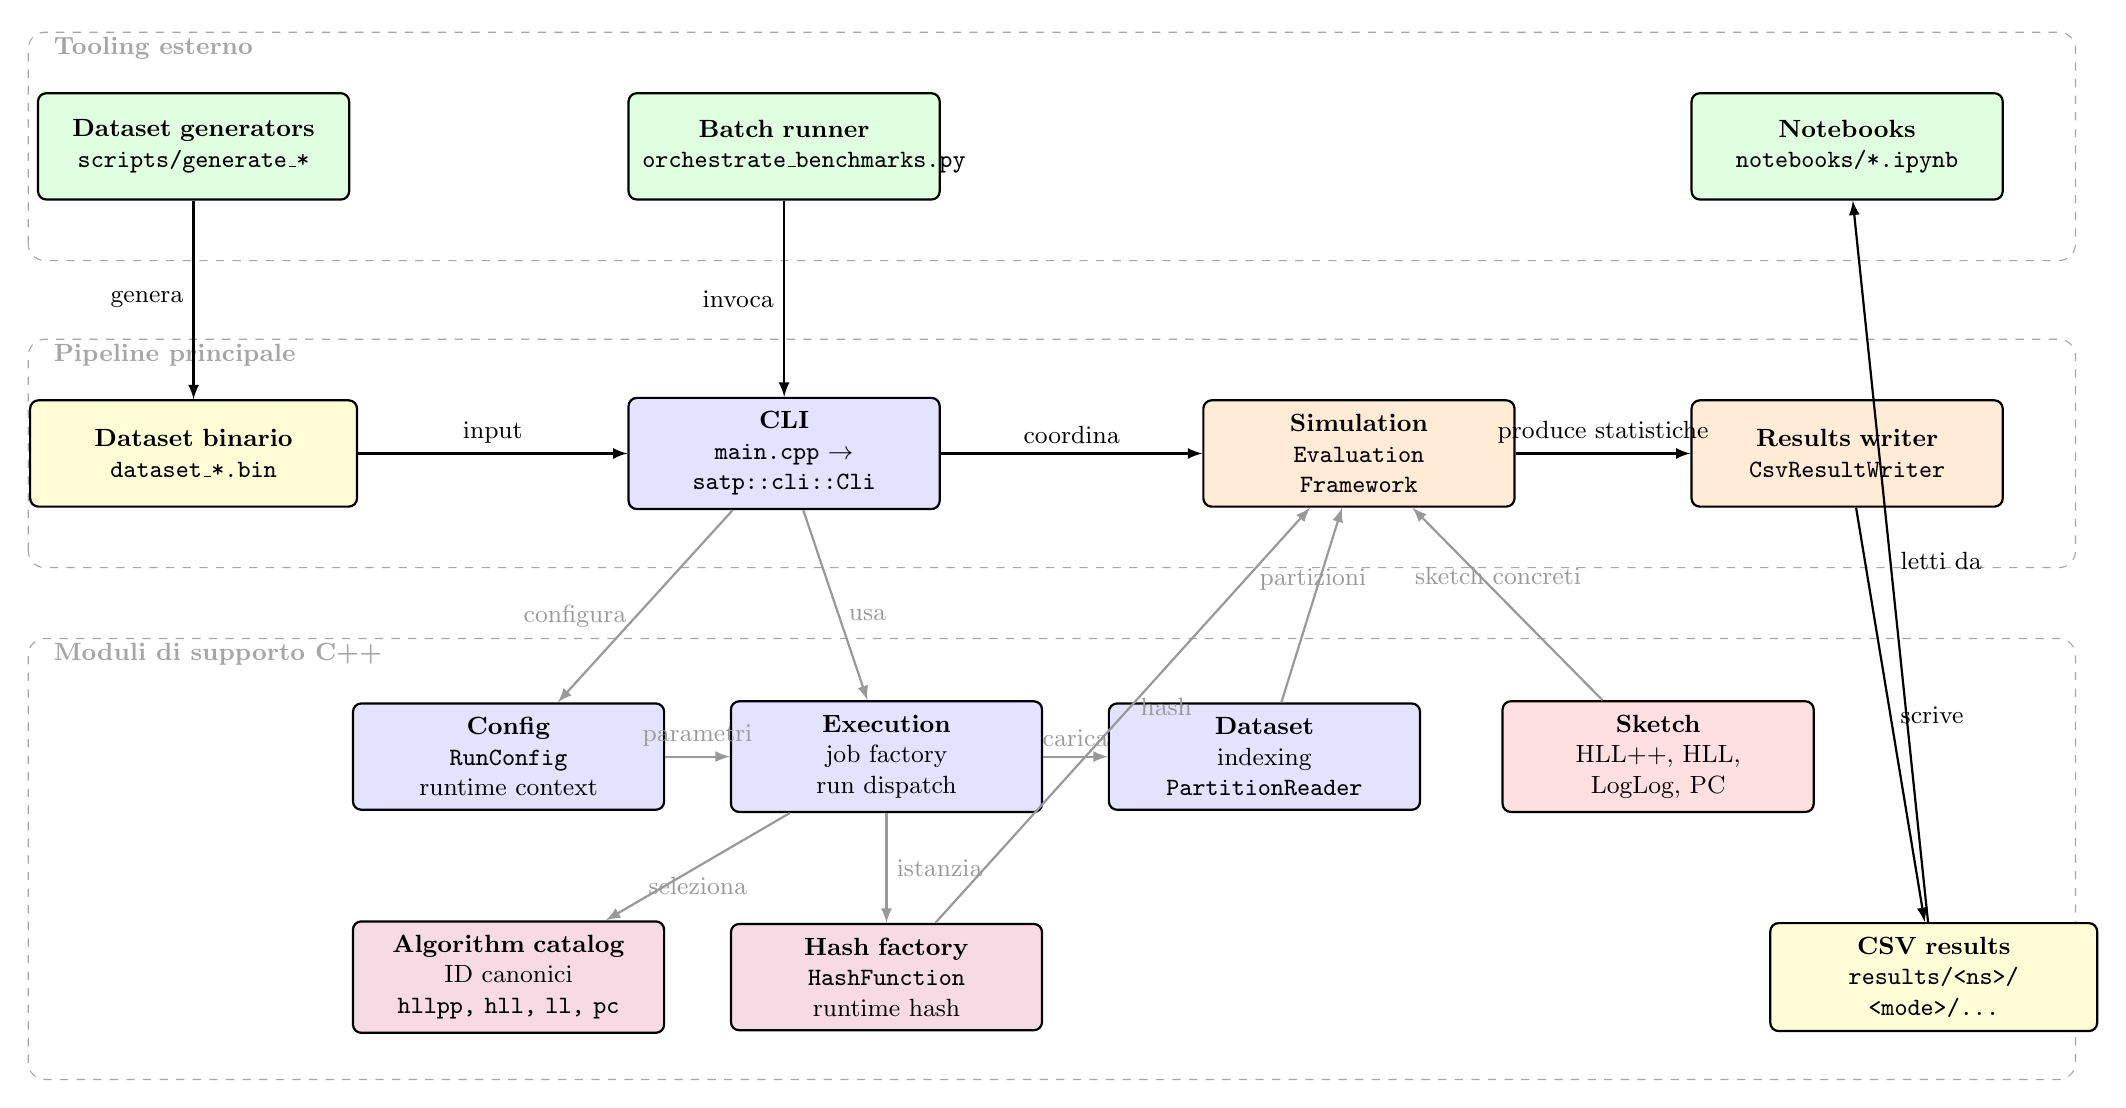
\begin{tikzpicture}[x=1cm,y=1cm,>=latex,font=\small]
    \tikzstyle{module}=[draw, rounded corners=3pt, thick, align=center,
        text width=3.6cm, minimum height=1.35cm, inner sep=5pt]
    \tikzstyle{artifact}=[draw, rounded corners=3pt, thick, align=center,
        text width=3.8cm, minimum height=1.35cm, inner sep=5pt]
    \tikzstyle{flow}=[->, thick]
    \tikzstyle{support}=[->, thick, gray!80]

    % Layer frames
    \draw[dashed, rounded corners=6pt, gray!70] (-2.1,7.3) rectangle (23.9,10.2);
    \node[anchor=west, gray!70] at (-1.9,10.0) {\textbf{Tooling esterno}};

    \draw[dashed, rounded corners=6pt, gray!70] (-2.1,3.4) rectangle (23.9,6.3);
    \node[anchor=west, gray!70] at (-1.9,6.1) {\textbf{Pipeline principale}};

    \draw[dashed, rounded corners=6pt, gray!70] (-2.1,-3.1) rectangle (23.9,2.5);
    \node[anchor=west, gray!70] at (-1.9,2.3) {\textbf{Moduli di supporto C++}};

    % External tooling
    \node[module, fill=green!12] (generators) at (0.0,8.75)
        {\textbf{Dataset generators}\\\texttt{scripts/generate\_*}};
    \node[module, fill=green!12] (orchestrator) at (7.5,8.75)
        {\textbf{Batch runner}\\\texttt{orchestrate\_benchmarks.py}};
    \node[module, fill=green!12] (notebooks) at (21.0,8.75)
        {\textbf{Notebooks}\\\texttt{notebooks/*.ipynb}};

    % Main pipeline
    \node[artifact, fill=yellow!16] (datasetfile) at (0.0,4.85)
        {\textbf{Dataset binario}\\\texttt{dataset\_*.bin}};
    \node[module, fill=blue!11] (cli) at (7.5,4.85)
        {\textbf{CLI}\\\texttt{main.cpp} $\rightarrow$ \texttt{satp::cli::Cli}};
    \node[module, fill=orange!16] (simulation) at (14.8,4.85)
        {\textbf{Simulation}\\\texttt{Evaluation}\\\texttt{Framework}};
    \node[module, fill=orange!16] (writer) at (21.0,4.85)
        {\textbf{Results writer}\\\texttt{CsvResultWriter}};

    % Support modules
    \node[module, fill=blue!11] (config) at (4.0,1.0)
        {\textbf{Config}\\\texttt{RunConfig}\\runtime context};
    \node[module, fill=blue!11] (execution) at (8.8,1.0)
        {\textbf{Execution}\\job factory\\run dispatch};
    \node[module, fill=blue!11] (dataset) at (13.6,1.0)
        {\textbf{Dataset}\\indexing\\\texttt{PartitionReader}};
    \node[module, fill=purple!14] (hashing) at (8.8,-1.8)
        {\textbf{Hash factory}\\\texttt{HashFunction}\\runtime hash};
    \node[module, fill=purple!14] (catalog) at (4.0,-1.8)
        {\textbf{Algorithm catalog}\\ID canonici\\\texttt{hllpp, hll, ll, pc}};
    \node[module, fill=red!12] (algorithms) at (18.6,1.0)
        {\textbf{Sketch}\\HLL++, HLL,\\LogLog, PC};
    \node[artifact, fill=yellow!16] (results) at (22.1,-1.8)
        {\textbf{CSV results}\\\texttt{results/<ns>/}\\\texttt{<mode>/...}};

    % Main flow
    \draw[flow] (generators) -- node[left, pos=0.5] {genera} (datasetfile);
    \draw[flow] (orchestrator) -- node[left, pos=0.5] {invoca} (cli);
    \draw[flow] (datasetfile) -- node[above, pos=0.5] {input} (cli);
    \draw[flow] (cli) -- node[above, pos=0.5] {coordina} (simulation);
    \draw[flow] (simulation) -- node[above, pos=0.5] {produce statistiche} (writer);
    \draw[flow] (writer) -- node[right, pos=0.5] {scrive} (results);
    \draw[flow] (results) -- node[right, pos=0.5] {letti da} (notebooks);

    % Support relations
    \draw[support] (cli) -- node[left, pos=0.55] {configura} (config);
    \draw[support] (cli) -- node[right, pos=0.55] {usa} (execution);
    \draw[support] (config) -- node[above, pos=0.5] {parametri} (execution);
    \draw[support] (execution) -- node[above, pos=0.5] {carica} (dataset);
    \draw[support] (execution) -- node[right, pos=0.5] {istanzia} (hashing);
    \draw[support] (execution) -- node[below, pos=0.5] {seleziona} (catalog);
    \draw[support] (dataset) -- node[above, pos=0.52] {partizioni} (simulation);
    \draw[support] (hashing) -- node[right, pos=0.52] {hash} (simulation);
    \draw[support] (algorithms) -- node[above, pos=0.55] {sketch concreti} (simulation);
\end{tikzpicture}
